\documentclass[a4paper,12pt]{report}
\usepackage{natbib}
\usepackage{packages/rapportutc}
\usepackage[nottoc, notlof, notlot]{tocbibind}
\usepackage{sidecap}
\usepackage{array}
\usepackage[linewidth=1pt]{mdframed}

\usepackage{packages/Sweave} %package d'affichage des codes R
\usepackage{amsmath, amsthm, amssymb, graphics, setspace} %packages de mathématiques
\usepackage{calc,enumitem}  % Mise en forme l'environnement itemsize description etc.
\usepackage{subfigure, wrapfig} % pour avoir plusieurs figures alignées  
\usepackage{color}
\usepackage{ae,aecompl}
\usepackage{pifont}
\usepackage{chemist} %formule chimique 
\usepackage{comment}
\usepackage{rotating}
\usepackage{hyperref}
\usepackage{listings}


%\usepackage{biblatex}

%%%%%%%%%%%%%%%%%%%%%%%%%%%%%%%%%%%%%%%%%%%%%%%%%%%%%%%%%%%%%%%%%%%%%%%%%%%% 

\title{TP 1 - Statistique descriptive, Analyse en composantes principales}
\author{LU Han - HAMONNAIS Raphaël}
\date{\today}

\uv{SY09}
\branche{Génie Informatique}
\filiere{Fouille de Données et Décisionnel}
%%%%%%%%%%%%%%%%%%%%%%%%%%%%%%%%%%%%%%%%%%%%%%%%%%%%%%%%%%%%%%%%%%%%%%%%%%%%

\begin{document}
\renewcommand{\labelitemi}{\large\textcolor{tatoebagreen}{\fg}}
\newgeometry{top=2.5cm,bottom=2cm,left=2cm,right=2cm}
\groovypdtitre
\restoregeometry % restaure la géométrie par défaut de latex

%%%%%%%%%%%%%%%%%%%%%%%%%%%%%%%%%%%%%%%%%%%%%%%%%%%%%%%%%%%%%%%%%%%%%%%%%%%% 

\tableofcontents

%%%%%%%%%%%%%%%%%%%%%%%%%%%%%%%%%%%%%%%%%%%%%%%%%%%%%%%%%%%%%%%%%%%%%%%%%%%%



\chapter{Statistique descriptive}

\section{Notes SY02 au semestre de printemps 2016}

\subsection{Analyse descriptive}

\paragraph{Description des données}


Le jeu de données contient des informations relatives aux 296 étudiants inscrits à l’UV SY02 au semestre de printemps 2016 ainsi que les résultats qu'ils ont obtenus. On a donc 296 mesures (individus de la population) représentés par onze variables~: 8 qualitatives et 3 quantitatives.\\
Liste des variables qualitatives~:
\begin{itemize}
	\item \textbf{nom} : nom de l'étudiant, au format texte (nons anonymisés, au format "Etu1, Etu2,~...").
	\item \textbf{specialite} : spécialité de l'étudiant, $\in$ \{GB, GI, GM, GP, GSM, GSU, HuTech, ISS, TC\}.
	\item \textbf{niveau} : le numéro du semestre actuel de l'étudiant, $ \in \{1,2,3,4,5,6\} $.
	\item \textbf{statut} : vaut $ \{UTC,Echange\} $ selon que c'est un étudiant de l'UTC ou bien un étudiant originaire d'une autre université effectuant une partie de ses études à l'UTC.
	\item \textbf{dernier.diplome.obtenu} : le dernier diplôme obtenu par l'étudiant, $\in$ \{AUTRE 1ER CYCLE, AUTRE 2E CYCLE AUTRE DIPLOME SUPERIEUR, BAC, BTS, CPGE, DEUG, DUT, ETRANGER SECONDAIRE, ETRANGER SUPERIEUR, INGENIEUR, LICENCE, NA's\}.
	\item \textbf{correcteur.median} et \textbf{correcteur.final} : le correcteur ayant corrigé la copie (nons anonymisés au format "Cor 1,~...").
	\item \textbf{resultat} Le résultat de l'étudiant, de \textit{A} à \textit{F} ou \textit{ABS} s'il a été absent à l'un des deux examens (final ou médian). \textit{F} et \textit{Fx} signifient que l'étudiant n'a pas obtenu l'UV, les autres notes qu'il l'a obtenue.
\end{itemize}
Liste des variables quantitatives~:
\begin{itemize}
	\item \textbf{note.median} : la note obtenue au médian ($ \in [0;20] $).
	\item \textbf{note.final} : la note obtenue au final ($ \in [0;20] $).
	\item \textbf{note.totale} : la moyenne des deux notes, pondérée par l'importance de chaque note.
\end{itemize}


\paragraph{Données manquantes}
On remarque qu'il manque certaines informations dans les données (R le spécifie avec le mot clé "\textit{NA's}" pour \textit{Not Available} en anglais).
\begin{itemize}
	\item Correcteur du médian et/ou du final~: élève absent au médian et/ou au final.
	\item Dernier diplôme obtenu~: donnée manquante pour les étudiants en échange.
	\item Note au médian et/ou au final~: donnée manquante pour les étudiants absents ou qui ont abandonné.
	\item Résultat~: donnée "manquante" pour R qui considère la valeur \textit{ABS} comme étant manquant car \textit{resultat} est une variable qualitative ordonnée et \textit{ABS} ne fait pas partie des différents niveau d'ordre. Représente donc des élèves absents qui n'ont pas obtenu l'UV.
\end{itemize}


\paragraph{Intuitions statistiques~: liens supposés entre les variables}
De manière logique, on pourrait penser que les notes entre le médian et le final sont liées, un élève bon au médian étant plus à même de réussir le final et inversement. De même, la formation d'origine de l'étudiant devrait fortement influencer l'obtention de l'UV. Un étudiant venant de tronc commun (diplôme d'origine BAC) a logiquement plus de change de réussir qu'un élève venant de DUT. Le correcteur ne devrait logiquement pas influencer les notes, la notion d'équité entre les copies étant très importante.




\subsection{Etude des liens statistique entre les variables}
On considère que les données ont été préalablement nettoyées en enlevant tous les étudiants absents, c'est à dire qui n'ont pas eu l'UV pour cause d'absence accidentelle ou d'abandon pur et simple.



Nous utiliserons le test d'indépendance du $\chi^2$ qui permet de vérifier l'indépendance de deux variables X et Y : 

\begin{itemize}
	\item Hypothèse nulle $H_{0}$~: les deux variables X et Y sont indépendantes.
	\item Hypothèse $H_{0}$~: les deux variables X et Y ne sont pas indépendantes.
	\item On rejette l'hypothèse nulle lorsque \textit{p-value}\footnote{Probabilité d'obtenir la même valeur (ou une valeur encore plus extrême) du test si l'hypothèse nulle était vraie} est inférieure ou égale à 0,05.
	\item Toutes les cases du tableau de contingence\footnote{Tableau à double entrée représentant les effectifs partiels des observations en fonction des variables X en ligne et Y en colonne} doivent avoir une valeur supérieure ou égale à 5.
\end{itemize}

\subsubsection{Lien entre le résultat et la formation d'origine de l'étudiant}

La première chose à faire est de nettoyer les données en supprimant les 6 étudiants dont le statut vaut \textit{Echange} car leur diplôme d'origine n'est pas renseigné.\\
Ensuite nous allons créer le tableau de contingence qui donne pour chaque valeur de la variable \textit{resultat} le nombre d'élèves ayant obtenu ce résultat en fonction de leur diplôme d'origine.

\begin{figure}[h]
	\centering
	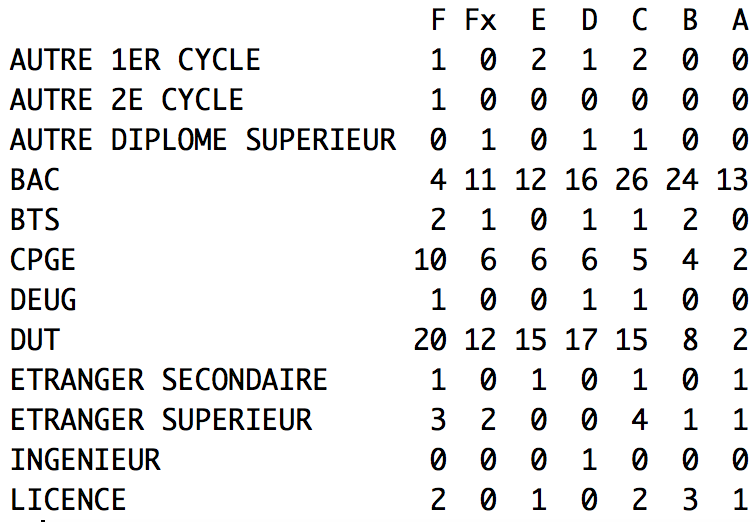
\includegraphics[width=0.7\linewidth]{img/1-1-2-Contingence-Result-Diplome-Origine}
	\caption[]{Tableau de contingence résultats vs. diplômes d'origine}
	\label{fig:1-1-2-contingence-result-diplome-origine}
\end{figure}

	
\end{document}